\chapter{P Versus NP}
\label{ch:pvsnp}

\noindent\textbf{Key Ideas.}
\begin{itemize}
  \item \textbf{P} = problems solvable in polynomial time; \textbf{NP} = problems whose solutions are verifiable in polynomial time.
  \item An \emph{NP-complete} problem is the hardest in NP: solving one in polynomial time solves all of them.
  \item The question P $\stackrel{?}{=}$ NP asks whether efficient verification implies efficient solution.
  \item Most experts believe P $\neq$ NP, but no proof exists.
\end{itemize}

\bigskip

\section{Introduction}

The P versus NP problem is widely regarded as the most important open question in computer science and one of the deepest in all of mathematics. It asks a deceptively simple question: \emph{if a solution to a problem can be verified quickly, can the solution itself be found quickly?}

More precisely, consider problems whose answers can be \emph{checked} in polynomial time---that is, problems for which a proposed answer can be confirmed by a fast algorithm. The class of such problems is called NP. The class P consists of problems that can be \emph{solved} in polynomial time. The question is whether every problem whose solution is quickly verifiable is also quickly solvable:
\[
\text{P} \stackrel{?}{=} \text{NP}.
\]

This question has extraordinary practical significance. Thousands of important problems across science, engineering, and industry---from scheduling airline crews, to designing computer chips, to predicting protein structures, to breaking cryptographic codes---are known to belong to NP. If P = NP, then efficient algorithms exist for all of them, and the consequences for science, technology, and security would be revolutionary. If P $\neq$ NP, as the vast majority of computer scientists believe, then some problems are fundamentally intractable: no amount of cleverness or computing power can make them tractable for large inputs, and we must settle for approximate solutions or accept exponential running times.

The problem was formally posed in a landmark 1971 paper by Stephen Cook, who proved that the Boolean satisfiability problem (SAT) is \emph{NP-complete}: it is among the hardest problems in NP, so that a polynomial-time algorithm for SAT would imply one for every problem in NP. Leonid Levin independently discovered the same result around the same time. In 2000, the Clay Mathematics Institute designated P versus NP as one of the seven Millennium Prize Problems, offering one million dollars for its resolution.

This chapter develops the theory of computational complexity from the ground up. We begin with models of computation and the definition of polynomial time, introduce the classes P and NP, study the phenomenon of NP-completeness, and then examine the profound consequences of each possible resolution. We discuss the major barrier results that explain why the problem has resisted all proof attempts, and survey the rich landscape of complexity classes beyond P and NP. The chapter concludes with exercises that invite the reader to engage directly with these ideas.

\section{Models of Computation}

To ask questions about what can be computed efficiently, we first need a precise model of computation. The answer must not depend on whether we use a laptop, a quantum computer, or an alien device---it must capture the \emph{intrinsic} difficulty of a problem.

\subsection{Turing Machines}

The foundational model of computation is the Turing machine, introduced by Alan Turing in 1936.

\begin{definition}[Deterministic Turing machine]
A \textbf{deterministic Turing machine} (DTM) is a 7-tuple $M = (Q, \Sigma, \Gamma, \delta, q_0, q_{\text{accept}}, q_{\text{reject}})$ where:
\begin{enumerate}
  \item $Q$ is a finite set of states,
  \item $\Sigma$ is the input alphabet (not containing the blank symbol $\sqcup$),
  \item $\Gamma \supseteq \Sigma \cup \{\sqcup\}$ is the tape alphabet,
  \item $\delta: Q \times \Gamma \to Q \times \Gamma \times \{L, R\}$ is the transition function,
  \item $q_0 \in Q$ is the start state,
  \item $q_{\text{accept}} \in Q$ is the accept state, and
  \item $q_{\text{reject}} \in Q$ is the reject state.
\end{enumerate}
\end{definition}

A DTM operates on a one-way infinite tape divided into cells, each holding a symbol from $\Gamma$. A head reads and writes symbols on the tape and moves left or right one cell at a time, governed by the transition function $\delta$. Computation begins in state $q_0$ with the input written on the tape and all other cells blank. The machine halts and \emph{accepts} if it enters $q_{\text{accept}}$, and halts and \emph{rejects} if it enters $q_{\text{reject}}$. For inputs not in the language, the machine may also loop forever.

\begin{definition}[Language recognized by a Turing machine]
A language $L \subseteq \Sigma^*$ is \textbf{decidable} if there exists a deterministic Turing machine $M$ such that for every string $x \in \Sigma^*$:
\begin{itemize}
  \item If $x \in L$, then $M$ accepts $x$.
  \item If $x \notin L$, then $M$ rejects $x$.
\end{itemize}
\end{definition}

\begin{example}
The language $\text{EVEN} = \{w \in \{0,1\}^* : |w| \text{ is even}\}$ is decidable. A Turing machine can scan the tape from left to right, toggling between two states as it reads each symbol, and accept if it is in the ``even'' state when the blank is reached.
\end{example}

\subsection{Non-Deterministic Turing Machines}

The class NP is most naturally defined in terms of non-deterministic computation.

\begin{definition}[Non-deterministic Turing machine]
A \textbf{non-deterministic Turing machine} (NTM) is defined identically to a DTM except that the transition function has the form $\delta: Q \times \Gamma \to \mathcal{P}(Q \times \Gamma \times \{L, R\})$, where $\mathcal{P}$ denotes the power set. At each step, the machine may \emph{choose} from a set of possible transitions.
\end{definition}

An NTM accepts an input $x$ if \emph{there exists} at least one computation path (sequence of non-deterministic choices) that leads to $q_{\text{accept}}$. Rejection requires \emph{all} computation paths to lead to $q_{\text{reject}}$ (or to loop forever).

Non-deterministic computation is not a physical device---no machine of this kind can actually be built. Rather, it is a mathematical tool: a problem belongs to NP precisely when a non-deterministic Turing machine can solve it in polynomial time.

\begin{remark}
The intuition behind non-determinism is sometimes described as ``guessing and checking.'' An NTM ``guesses'' the correct certificate and then ``verifies'' it deterministically. This intuition is made precise in the verifier definition of NP (Section~3.4).
\end{remark}

\subsection{The Church--Turing Thesis}

In the 1930s, Alonzo Church developed the lambda calculus and Alan Turing developed the Turing machine, independently arriving at the same class of computable functions. This led to a fundamental principle:

\begin{thesis}[Church--Turing thesis]
Every function that is intuitively computable is computable by a Turing machine.
\end{thesis}

The Church--Turing thesis is not a theorem---it cannot be proved because ``intuitively computable'' is an informal notion. However, every reasonable model of computation that has been proposed (lambda calculus, recursive functions, register machines, cellular automata) has been shown to compute exactly the same class of functions as Turing machines. This universal agreement provides overwhelming evidence for the thesis.

For our purposes, the stronger \textit{extended Church--Turing thesis} is relevant:

\begin{thesis}[Extended Church--Turing thesis]
Any function computable by any physical device in polynomial time is computable by a deterministic Turing machine in polynomial time (up to a polynomial overhead).
\end{thesis}

This thesis is more controversial. Quantum computing, if scalable, would violate it, since quantum computers can solve certain problems (such as integer factorization) in polynomial time while no efficient classical algorithm is known. For classical computation, however, the extended thesis is widely accepted and justifies the use of Turing machines as the benchmark for efficiency.

\subsection{The RAM Model}

In practice, algorithms are analyzed not on Turing machines but on the \textbf{random-access machine} (RAM) model. A RAM consists of:
\begin{itemize}
  \item An unbounded set of registers, each holding an arbitrarily large integer.
  \item A program (finite sequence of instructions) that can read from and write to registers, perform arithmetic, and branch conditionally.
  \item Each basic operation (addition, comparison, memory access) costs one unit of time.
\end{itemize}

The RAM model is more realistic than Turing machines for analyzing algorithms on actual computers. Crucially, under the extended Church--Turing thesis, the two models are polynomially equivalent:

\begin{proposition}
If a language $L$ is decidable by a DTM in time $O(T(n))$, then $L$ is decidable by a RAM in time $O(T(n))$. Conversely, if a RAM decides $L$ in time $O(T(n))$ with integers of polynomial bit-length, then a DTM decides $L$ in time $O(T(n)^c)$ for some constant $c$.
\end{proposition}

This means that for classifying problems into P, NP, and so on, the choice of model does not matter: the classes are invariant under polynomial-time transformations between models. For analyzing the running time of specific algorithms, the RAM model is typically used because it closely approximates real computers.

\subsection{Why Turing Machines?}

Turing machines are the standard model for complexity theory for several reasons:
\begin{enumerate}
  \item \textbf{Simplicity:} The model is simple enough for rigorous analysis. Time and space are unambiguous.
  \item \textbf{Universality:} The Church--Turing thesis ensures no model is more powerful for computability.
  \item \textbf{Polynomial invariance:} For complexity classes, the choice of reasonable model does not change the class. A problem in P under one model is in P under all reasonable models.
  \item \textbf{Historical priority:} Turing's analysis of computability laid the groundwork for all of complexity theory.
\end{enumerate}

\subsection{Time Complexity and Big-O Notation}

To measure the efficiency of an algorithm, we count the number of steps it takes as a function of the input size.

\begin{definition}[Time complexity]
Let $M$ be a deterministic Turing machine that halts on all inputs. The \textbf{time complexity} (or \textbf{running time}) of $M$ is the function $T: \mathbb{N} \to \mathbb{N}$ where $T(n)$ is the maximum number of steps $M$ takes on any input of length $n$.
\end{definition}

Because the exact number of steps depends on implementation details, we use asymptotic notation to abstract away constants.

\begin{definition}[Big-O notation]
Let $f, g: \mathbb{N} \to \mathbb{R}_{\geq 0}$. We write $f(n) = O(g(n))$ if there exist positive constants $c$ and $n_0$ such that $f(n) \leq c \cdot g(n)$ for all $n \geq n_0$.
\end{definition}

\begin{definition}[Omega and Theta notation]
\begin{itemize}
  \item $f(n) = \Omega(g(n))$ if $g(n) = O(f(n))$.
  \item $f(n) = \Theta(g(n))$ if $f(n) = O(g(n))$ and $g(n) = O(f(n))$.
\end{itemize}
\end{definition}

\begin{example}
If an algorithm performs $3n^2 + 7n + 12$ operations on inputs of size $n$, then its running time is $O(n^2)$, $\Omega(n^2)$, and $\Theta(n^2)$.
\end{example}

\begin{example}
Merge sort runs in $O(n \log n)$ time. Insertion sort runs in $O(n^2)$ time in the worst case but $O(n)$ in the best case.
\end{example}

The use of $O$-notation reflects the principle that what matters for classifying problems is the \emph{growth rate} of the running time, not the exact number of steps. An algorithm running in $10^{100} \cdot n$ steps is in the same complexity class as one running in $3n + 5$ steps: both are $O(n)$. The constant factors are absorbed.

\begin{remark}
In complexity theory, the input size $n$ is the length of the input measured in bits. For an integer $N$, the input size is $\Theta(\log N)$ bits. For a graph with $V$ vertices and $E$ edges, the input size is $\Theta(V + E)$ bits. This distinction is critical: a $O(N)$-time algorithm for a problem with integer input $N$ is actually $O(2^n)$ in the input size $n = \log_2 N$, which is exponential.
\end{remark}

\section{The Class P}

\subsection{Formal Definition}

\begin{definition}[P]
The complexity class \textbf{P} is the set of all languages (decision problems) $L \subseteq \{0,1\}^*$ for which there exists a deterministic Turing machine $M$ and a polynomial $p$ such that $M$ decides $L$ in time $O(p(n))$, where $n = |x|$ is the length of the input.
\end{definition}

Equivalently, $L \in \text{P}$ if and only if there is an algorithm for $L$ whose worst-case running time is bounded by a polynomial in the input size. The class P represents the informal notion of ``efficiently solvable'' or ``tractable'' problems.

\begin{checkyou}
\begin{enumerate}
  \item Explain why merge sort's $O(n \log n)$ running time places it in P, but an $O(2^n)$ algorithm would not.
  \item Is $O(n^{100})$ tractable in practice? Does this change its membership in P?
\end{enumerate}
\end{checkyou}

\begin{remark}
The class P is independent of the specific model of computation used (DTM, RAM, etc.) because all standard models simulate each other with at most polynomial overhead. This is a consequence of the extended Church--Turing thesis and the polynomial simulation between models.
\end{remark}

\subsection{Examples of Problems in P}

We now survey several important problems that are known to lie in P.

\begin{example}[Shortest path]
\textbf{Problem:} Given a weighted graph $G$ with non-negative edge weights and two vertices $s$ and $t$, find the shortest path from $s$ to $t$.
\par\textbf{Algorithm:} Dijkstra's algorithm, running in $O((V + E) \log V)$ time using a priority queue.
\end{example}

\begin{example}[Minimum spanning tree]
\textbf{Problem:} Given a weighted graph $G$, find a spanning tree of minimum total weight.
\par\textbf{Algorithm:} Kruskal's or Prim's algorithm, running in $O(E \log V)$ time.
\end{example}

\begin{example}[Primality testing]
\textbf{Problem:} Given an integer $n$, is $n$ prime?
\par\textbf{Algorithm:} The AKS primality test (Agrawal, Kayal, and Saxena, 2002) runs in $\tilde{O}((\log n)^6)$ time. Earlier probabilistic algorithms (Miller--Rabin, Solovay--Strassen) were faster but only correct with high probability.
\end{example}

The AKS result resolved a long-standing open question. For decades, primality testing was one of the most prominent problems believed to be in P but not yet proved so.

\begin{example}[Eulerian circuit]
\textbf{Problem:} Given a connected graph $G$, does $G$ contain a closed walk that traverses every edge exactly once?
\par\textbf{Algorithm:} By Euler's theorem (1736), $G$ has an Eulerian circuit if and only if every vertex has even degree. Checking this takes $O(V + E)$ time.
\end{example}

\begin{example}[2-SAT]
\textbf{Problem:} Given a Boolean formula in conjunctive normal form (CNF) where each clause has at most two literals, is the formula satisfiable?
\par\textbf{Algorithm:} 2-SAT can be solved in $O(n + m)$ time (where $n$ is the number of variables and $m$ is the number of clauses) by constructing an implication graph and computing strongly connected components. A formula is satisfiable if and only if no variable and its negation belong to the same strongly connected component.
\end{example}

Compare this with 3-SAT (where clauses have exactly three literals), which is NP-complete. The jump from two to three literals per clause is the threshold where tractability appears to break down.

\begin{example}[Linear programming]
\textbf{Problem:} Given a system of linear inequalities $Ax \leq b$ with rational entries, does there exist a rational vector $x$ satisfying all constraints?
\par\textbf{Algorithm:} The ellipsoid method (Khachiyan, 1979) and interior-point methods (Karmarkar, 1984) solve linear programming in polynomial time.
\end{example}

Linear programming is a remarkable case: the problem was central to operations research for decades, and practical algorithms (the simplex method) worked well in practice but had exponential worst-case complexity. The discovery of polynomial-time algorithms was a major theoretical achievement, though the simplex method remains faster in practice for most instances.

\begin{example}[Network flow]
\textbf{Problem:} Given a directed graph with edge capacities and a source-sink pair, find the maximum flow.
\par\textbf{Algorithm:} The push-relabel algorithm of Goldberg and Tarjan runs in $O(V \cdot E \log(V^2/E))$ time.
\end{example}

\subsection{Polynomial vs.\ Exponential Time}

The distinction between polynomial and exponential time is the central dividing line in complexity theory.

\begin{table}[ht]
\centering
\begin{tabular}{lrc}
\toprule
\textbf{Function} & \textbf{Input size $n$} & \textbf{Operations for $n = 50$} \\
\midrule
$n$ & 50 & $50$ \\
$n^2$ & 50 & $2{,}500$ \\
$n^3$ & 50 & $125{,}000$ \\
$n^5$ & 50 & $3.1 \times 10^8$ \\
$2^n$ & 50 & $1.1 \times 10^{15}$ \\
$n!$ & 50 & $3.0 \times 10^{64}$ \\
\bottomrule
\end{tabular}
\caption{Growth rates of common functions. Even for moderate input sizes, exponential functions vastly exceed polynomial ones.}
\label{tab:growth}
\end{table}

As Table~\ref{tab:growth} illustrates, the gap between polynomial and exponential growth is enormous. A problem with a $2^n$-time algorithm is infeasible for inputs of even a few hundred bits, while a problem with an $n^{10}$-time algorithm is (in principle) tractable for inputs of thousands of bits.

\begin{remark}
Polynomial time is sometimes criticized as an imperfect proxy for ``tractability.'' An algorithm with running time $n^{100}$ is technically polynomial but practically useless. Conversely, some exponential algorithms (e.g., for the traveling salesman problem with $n \le 30$ cities) work well in practice. Despite these caveats, the polynomial-time criterion has proven to be a robust and productive dividing line in complexity theory, and no alternative has gained broad acceptance.
\end{remark}

\subsection{What ``Efficient'' Means}

In theoretical computer science, ``efficient'' is a technical term meaning ``computable in polynomial time.'' This identification is motivated by several observations:

\begin{enumerate}
  \item \textbf{Closure under composition:} If algorithm $A$ runs in time $n^{c_1}$ and algorithm $B$ runs in time $n^{c_2}$, then running $B$ on the output of $A$ gives a total running time of $O(n^{c_1 \cdot c_2})$, which is still polynomial. This closure property fails for exponential functions ($2^{2^n}$ is doubly exponential).
  \item \textbf{Robustness under modeling:} Polynomial time is invariant under polynomial changes in the model of computation, making it a natural notion of efficiency.
  \item \textbf{Practical correlation:} Problems with polynomial-time algorithms tend to be solvable in practice for reasonable input sizes, while problems requiring super-polynomial time tend to become infeasible quickly.
\end{enumerate}

\section{The Class NP}

\subsection{The Verifier Definition}

The class NP can be defined in several equivalent ways. The most intuitive is the \emph{verifier} definition.

\begin{definition}[NP via verifiers]
A language $L$ is in \textbf{NP} if there exists a deterministic polynomial-time Turing machine $V$ (the \textbf{verifier}) and a polynomial $q$ such that for every $x \in \{0,1\}^*$:
\begin{itemize}
  \item If $x \in L$, there exists a string $y \in \{0,1\}^{*}$ with $|y| \leq q(|x|)$ such that $V(x, y) = \text{accept}$.
  \item If $x \notin L$, then for all strings $y$ with $|y| \leq q(|x|)$, $V(x, y) = \text{reject}$.
\end{itemize}
The string $y$ is called a \textbf{certificate} (or \textbf{witness}).
\end{definition}

In other words, $L \in \text{NP}$ means: if the answer is ``yes,'' there exists a short proof (certificate) that a fast algorithm can check. If the answer is ``no,'' no such proof exists.

\begin{checkyou}
\begin{enumerate}
  \item Is the certificate for a ``no'' instance required to not exist, or just to be unverifiable?
  \item For the Hamiltonian cycle problem, what is the certificate and why is verification fast even though finding the certificate may be hard?
\end{enumerate}
\end{checkyou}

\begin{remark}
The polynomial bound on the certificate length is essential. Without it, any decidable problem could be trivially placed in NP by using the entire computation history as a certificate.
\end{remark}

\subsection{Non-Deterministic Turing Machine Definition}

\begin{definition}[NP via NTMs]
A language $L$ is in \textbf{NP} if there exists a non-deterministic Turing machine $M$ and a polynomial $p$ such that for every $x \in \{0,1\}^*$:
\begin{itemize}
  \item If $x \in L$, then at least one computation path of $M$ on input $x$ leads to $q_{\text{accept}}$ within $p(|x|)$ steps.
  \item If $x \notin L$, then no computation path of $M$ on input $x$ leads to $q_{\text{accept}}$ within $p(|x|)$ steps.
\end{itemize}
\end{definition}

\begin{proposition}
The two definitions of NP (verifier and NTM) are equivalent.
\end{proposition}

\begin{proof}[Proof sketch]
($\Rightarrow$) Given an NTM $M$ that decides $L$ in non-deterministic polynomial time, construct a verifier $V$ that, on input $(x, y)$, interprets $y$ as a sequence of non-deterministic choices and simulates $M$ on $x$ using those choices. $V$ accepts if $M$ reaches $q_{\text{accept}}$.

($\Leftarrow$) Given a verifier $V$, construct an NTM $M$ that on input $x$, non-deterministically guesses a certificate $y$ (bit by bit) and then runs $V$ on $(x, y)$. If $V$ accepts, $M$ accepts.
\end{proof}

\subsection{Examples of Problems in NP}

\begin{example}[Boolean satisfiability (SAT)]
\textbf{Problem:} Given a Boolean formula $\phi$ over variables $x_1, \ldots, x_n$, is there an assignment of truth values making $\phi$ true?
\par\textbf{Certificate:} A satisfying assignment $(b_1, \ldots, b_n) \in \{0,1\}^n$.
\par\textbf{Verification:} Substitute the values and evaluate the formula. This takes $O(n)$ time.
\end{example}

\begin{example}[3-SAT]
\textbf{Problem:} SAT where each clause has exactly three literals (e.g., $(x_1 \lor \bar{x}_2 \lor x_3) \land (\bar{x}_1 \lor x_2 \lor x_3) \land \cdots$).
\par\textbf{Certificate and verification:} Identical to SAT. 3-SAT $\in$ NP.
\end{example}

\begin{example}[Hamiltonian cycle]
\textbf{Problem:} Given a graph $G = (V, E)$, does $G$ contain a cycle that visits every vertex exactly once?
\par\textbf{Certificate:} An ordering $v_1, v_2, \ldots, v_n$ of the vertices.
\par\textbf{Verification:} Check that each consecutive pair $(v_i, v_{i+1})$ is connected by an edge, and that $(v_n, v_1)$ is connected. This takes $O(n)$ time.
\end{example}

\begin{example}[Traveling salesman problem (TSP)]
\textbf{Problem:} Given $n$ cities with pairwise distances and a bound $B$, is there a tour (Hamiltonian cycle) of total length at most $B$?
\par\textbf{Certificate:} A permutation of the cities.
\par\textbf{Verification:} Sum the distances and compare to $B$. This takes $O(n)$ time.
\end{example}

\begin{example}[$k$-coloring]
\textbf{Problem:} Given a graph $G$ and an integer $k \geq 3$, can the vertices of $G$ be colored with $k$ colors so that no two adjacent vertices share a color?
\par\textbf{Certificate:} A coloring $c: V \to \{1, \ldots, k\}$.
\par\textbf{Verification:} Check that for every edge $(u,v) \in E$, $c(u) \neq c(v)$. This takes $O(|E|)$ time.
\end{example}

\begin{example}[Subset sum]
\textbf{Problem:} Given a set of integers $S = \{a_1, \ldots, a_n\}$ and a target $t$, is there a subset of $S$ summing to $t$?
\par\textbf{Certificate:} A subset $S' \subseteq S$.
\par\textbf{Verification:} Sum the elements of $S'$ and check if it equals $t$. This takes $O(n)$ time.
\end{example}

\begin{example}[Integer factorization]
\textbf{Problem:} Given an integer $n$, is $n$ composite (i.e., does $n$ have a non-trivial factor)?
\par\textbf{Certificate:} A factor $d$ with $1 < d < n$ and $d \mid n$.
\par\textbf{Verification:} Check that $d \mid n$ by computing $n \bmod d$. This takes $O(\log^2 n)$ time (polynomial in the input size).
\end{example}

Integer factorization is notable because it is believed to be in NP \textbackslash P (not solvable in polynomial time) yet is not believed to be NP-complete. If it were NP-complete, the polynomial hierarchy would collapse (see Section~3.10). This makes factorization a candidate for so-called NP-intermediate problems (see Section~3.8).

\subsection{Relationship P $\subseteq$ NP}

\begin{proposition}
$\text{P} \subseteq \text{NP}$.
\end{proposition}

\begin{proof}
If $L \in \text{P}$, then there is a deterministic polynomial-time algorithm $A$ that decides $L$. Construct a verifier $V$ that ignores its certificate and simply runs $A$ on the input. Then $x \in L$ iff $V(x, \epsilon)$ accepts, and $x \notin L$ iff $V(x, \epsilon)$ rejects. Since $A$ runs in polynomial time, so does $V$.
\end{proof}

The profound question is whether the inclusion is strict: does $\text{P} \subsetneq \text{NP}$?

\begin{figure}[htbp]
\centering
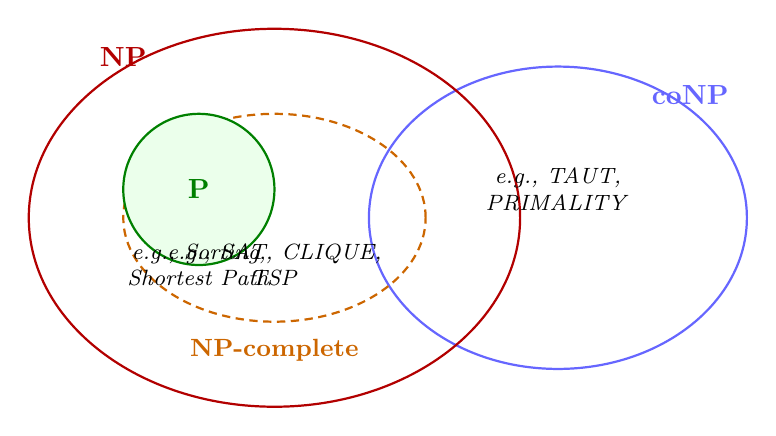
\begin{tikzpicture}[scale=1.2]
  % coNP circle (overlapping with NP)
  \draw[thick, blue!60] (2.2,0) ellipse (2.0 and 1.6);
  \node[blue!60, font=\bfseries] at (3.6,1.3) {coNP};
  % NP circle
  \draw[thick, red!70!black] (-0.8,0) ellipse (2.6 and 2.0);
  \node[red!70!black, font=\bfseries] at (-2.4,1.7) {NP};
  % NP-complete region (inside NP, outside P)
  \draw[thick, densely dashed, orange!80!black] (-0.8,0) ellipse (1.6 and 1.1);
  \node[orange!80!black, font=\small\bfseries] at (-0.8,-1.4) {NP-complete};
  % P circle (inside NP)
  \draw[thick, green!50!black, fill=green!8] (-1.6,0.3) circle (0.8);
  \node[green!50!black, font=\bfseries] at (-1.6,0.3) {P};
  % Labels
  \node[font=\footnotesize, align=center] at (-1.6,-0.5) {\textit{e.g., Sorting,}\\\textit{Shortest Path}};
  \node[font=\footnotesize, align=center] at (-0.8,-0.5) {\textit{e.g., SAT, CLIQUE,}\\\textit{TSP}};
  \node[font=\footnotesize, align=center] at (2.2,0.3) {\textit{e.g., TAUT,}\\\textit{PRIMALITY}};
\end{tikzpicture}
\caption{The relationship between the complexity classes P, NP, coNP, and NP-complete. If P $\neq$ NP, the NP-complete problems form a region inside NP but outside P. The class coNP overlaps with NP but is believed to be distinct from it.}
\label{fig:venn-complexity}
\end{figure}

\section{NP-Completeness}

The concept of NP-completeness is the central organizing principle of complexity theory. It identifies the \emph{hardest} problems in NP and shows that solving any one of them efficiently would solve them all.

\subsection{Polynomial-Time Reductions}

To formalize the idea that one problem is ``at least as hard as'' another, we use reductions.

\begin{definition}[Polynomial-time mapping reduction]
A language $A$ is \textbf{polynomial-time reducible} to a language $B$, written $A \leq_p B$, if there exists a polynomial-time computable function $f: \{0,1\}^* \to \{0,1\}^*$ such that for all $x \in \{0,1\}^*$:
\[
x \in A \iff f(x) \in B.
\]
The function $f$ is called the \textbf{reduction}.
\end{definition}

\begin{remark}
If $A \leq_p B$ and $B \in \text{P}$, then $A \in \text{P}$. Indeed, to decide $x \in A$, compute $f(x)$ (in polynomial time) and then decide whether $f(x) \in B$ (in polynomial time). The composition is polynomial time.
\end{remark}

\begin{corollary}
If $A \leq_p B$ and $A \notin \text{P}$, then $B \notin \text{P}$.
\end{corollary}

This contrapositive is the form most often used: if we know a problem $A$ is not in P, and $A \leq_p B$, then $B$ is also not in P. In particular, if $A$ is NP-complete and $A \leq_p B$ with $B \in \text{NP}$, then $B$ is NP-complete.

\subsection{Definition of NP-Completeness}

\begin{definition}[NP-complete]
A language $B$ is \textbf{NP-complete} if:
\begin{enumerate}
  \item $B \in \text{NP}$, and
  \item For every language $A \in \text{NP}$, $A \leq_p B$.
\end{enumerate}
\end{definition}

An NP-complete problem is simultaneously in NP and at least as hard as every problem in NP. If any NP-complete problem is in P, then $\text{P} = \text{NP}$.

\begin{checkyou}
\begin{enumerate}
  \item Give an example of a problem that is NP-hard but not in NP.
  \item Why can't an NP-hard problem outside NP be NP-complete?
\end{enumerate}
\end{checkyou}

\begin{remark}
Before Cook's 1971 paper, it was not even clear that NP-complete problems \emph{existed}. The Cook--Levin theorem settled this question by exhibiting the first NP-complete problem.
\end{remark}

\subsection{The Cook--Levin Theorem}

The Cook--Levin theorem is one of the most important results in the history of computer science.

\begin{theorem}[Cook--Levin, 1971]
SAT is NP-complete.
\end{theorem}

The theorem was proved independently by Stephen Cook (1971) and Leonid Levin (1973).

\begin{proof}[Proof sketch]
We must show that for every language $A \in \text{NP}$, $A \leq_p \text{SAT}$.

Let $M$ be a deterministic Turing machine that verifies $A$ in polynomial time $p(n)$. Given an input $x$ of length $n$, we construct a Boolean formula $\phi_x$ such that $\phi_x$ is satisfiable if and only if $M$ accepts $x$ (with some certificate).

The construction proceeds as follows. We encode the computation of $M$ on input $x$ using Boolean variables:

\begin{enumerate}
  \item \textbf{Configuration variables.} For each time step $t \in \{0, 1, \ldots, p(n)\}$, tape position $j \in \{0, 1, \ldots, p(n)\}$, and symbol $s \in \Gamma$, define a Boolean variable $\text{cell}(t, j, s)$ that is true iff the tape cell $j$ contains symbol $s$ at time $t$.

  \item \textbf{State variables.} For each time step $t$ and state $q \in Q$, define $\text{state}(t, q)$ that is true iff $M$ is in state $q$ at time $t$.

  \item \textbf{Head position variables.} For each time step $t$ and position $j$, define $\text{head}(t, j)$ that is true iff the head is at position $j$ at time $t$.
\end{enumerate}

The formula $\phi_x$ is a conjunction of clauses encoding:
\begin{itemize}
  \item \textbf{Initial configuration:} At time $t = 0$, the tape contains $x$, the head is at position 0, and $M$ is in state $q_0$.
  \item \textbf{Uniqueness:} At each time step, each cell contains exactly one symbol, the head is at exactly one position, and the machine is in exactly one state.
  \item \textbf{Transition correctness:} For each time step $t$ and position $j$, if the machine is in state $q$ reading symbol $s$ at position $j$ at time $t$, then at time $t+1$, the state, head position, and tape contents are consistent with the transition function $\delta(q, s)$.
  \item \textbf{Acceptance:} At some time step $t \leq p(n)$, the machine enters state $q_{\text{accept}}$.
\end{itemize}

Each of these conditions can be expressed as a Boolean formula of size $O(p(n)^2)$ (polynomial in $n$). The variables and clauses use a finite number of different sub-formulas, repeated for each time step and tape position. The key insight is that the \emph{locality} of the Turing machine transition function (it depends only on the current state and the symbol under the head) means each clause involves only a bounded number of variables.

Therefore, $\phi_x$ has $O(p(n)^2)$ variables and $O(p(n)^2)$ clauses, and can be constructed from $x$ in polynomial time. By construction, $\phi_x$ is satisfiable if and only if there exists a certificate causing $M$ to accept $x$, i.e., $x \in A$.
\end{proof}

\begin{remark}
The Cook--Levin theorem shows that the abstract computational process of a Turing machine can be ``compiled'' into a Boolean formula. The satisfiability of this formula precisely captures whether the computation accepts. This reduction is \emph{parsimonious}: the number of satisfying assignments equals the number of accepting computation paths.
\end{remark}

\begin{figure}[htbp]
\centering
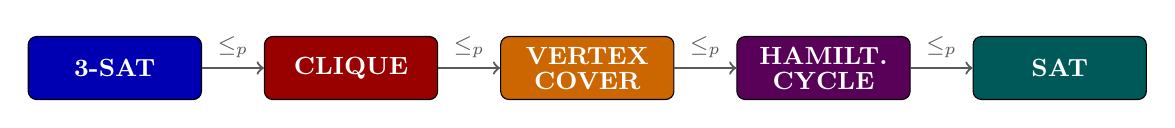
\begin{tikzpicture}[
  box/.style={draw, rounded corners=3pt, minimum width=2.2cm, minimum height=0.8cm,
              font=\small\bfseries, text=white, align=center},
  arr/.style={->, thick, gray!70!black}
]
  \node[box, fill=blue!70!black] (sat) at (0,0) {3-SAT};
  \node[box, fill=red!60!black] (clique) at (3,0) {CLIQUE};
  \node[box, fill=orange!80!black] (vc) at (6,0) {VERTEX\\[-2pt] COVER};
  \node[box, fill=violet!70!black] (hc) at (9,0) {HAMILT.\\[-2pt] CYCLE};
  \node[box, fill=teal!70!black] (sat2) at (12,0) {SAT};

  \draw[arr] (sat) -- node[above, font=\footnotesize] {$\leq_p$} (clique);
  \draw[arr] (clique) -- node[above, font=\footnotesize] {$\leq_p$} (vc);
  \draw[arr] (vc) -- node[above, font=\footnotesize] {$\leq_p$} (hc);
  \draw[arr] (hc) -- node[above, font=\footnotesize] {$\leq_p$} (sat2);
\end{tikzpicture}
\caption{A chain of polynomial-time reductions among NP-complete problems. Each arrow $A \leq_p B$ means that $A$ can be reduced to $B$ in polynomial time, so $B$ is at least as hard as $A$. Since SAT is NP-complete, all these problems are equivalent in difficulty.}
\label{fig:reduction-chain}
\end{figure}

\begin{checkyou}
\begin{enumerate}
  \item Why does Cook--Levin prove NP-completeness rather than just NP-hardness?
  \item Cook's proof reduces any NP language to SAT. What would it take to prove a different problem NP-complete without going through SAT?
\end{enumerate}
\end{checkyou}

\subsection{Karp's 21 NP-Complete Problems}

After Cook established that SAT is NP-complete, Richard Karp (1972) showed that 21 natural problems from diverse areas of mathematics and computer science are NP-complete, by exhibiting polynomial-time reductions from SAT to each of them. These include:

\begin{itemize}
  \item \textbf{3-SAT:} SAT restricted to clauses of exactly three literals.
  \item \textbf{CLIQUE:} Given a graph $G$ and integer $k$, does $G$ contain a complete subgraph on $k$ vertices?
  \item \textbf{VERTEX COVER:} Given a graph $G$ and integer $k$, is there a set of $k$ vertices touching every edge?
  \item \textbf{INDEPENDENT SET:} Given a graph $G$ and integer $k$, is there a set of $k$ pairwise non-adjacent vertices?
  \item \textbf{HAMILTONIAN CYCLE:} Given a graph $G$, does $G$ contain a cycle visiting every vertex exactly once?
  \item \textbf{HAMILTONIAN PATH:} Given a graph $G$, does $G$ contain a path visiting every vertex exactly once?
  \item \textbf{TSP (decision):} Given cities, distances, and a bound $B$, is there a tour of length $\leq B$?
  \item \textbf{$k$-COLORING:} Given a graph $G$ and $k \geq 3$, can $G$ be $k$-colored?
  \item \textbf{SUBSET SUM:} Given integers $a_1, \ldots, a_n$ and target $t$, is there a subset summing to $t$?
  \item \textbf{PARTITION:} Given integers $a_1, \ldots, a_n$, can they be partitioned into two equal-sum subsets?
  \item \textbf{3-DIMENSIONAL MATCHING:} Given three sets $X, Y, Z$ of equal size and triples $T \subseteq X \times Y \times Z$, is there a matching covering all elements?
  \item \textbf{SET COVER:} Given a universe $U$ and sets $S_1, \ldots, S_m \subseteq U$, and integer $k$, can $U$ be covered by $k$ sets?
  \item \textbf{KNAPSACK (decision):} Given items with weights and values, a capacity $W$, and a target $V$, is there a subset of total weight $\leq W$ and value $\geq V$?
  \item \textbf{INTEGER PROGRAMMING:} Given an integer matrix $A$ and vectors $b, c$, does $Ax \leq b$ have an integer solution $x$ with $c^T x \geq k$?
\end{itemize}

The proof technique is always the same: given an instance of SAT (or 3-SAT), construct in polynomial time an instance of the target problem such that the SAT instance is satisfiable iff the target instance is a ``yes'' instance.

\subsection{Example Reductions}

We illustrate the technique with two concrete reductions.

\subsubsection*{Reduction: 3-SAT $\leq_p$ CLIQUE}

Given a 3-SAT formula $\phi$ with $k$ clauses $C_1, \ldots, C_k$, construct a graph $G$ as follows:
\begin{enumerate}
  \item For each clause $C_i$ and each literal $\ell$ in $C_i$, create a vertex $v_{i,\ell}$.
  \item Connect $v_{i,\ell}$ to $v_{j,\ell'}$ with an edge if $i \neq j$ and the literals $\ell$ and $\ell'$ are not complementary (i.e., not $x$ and $\bar{x}$).
\end{enumerate}

\textbf{Claim:} $\phi$ is satisfiable iff $G$ has a clique of size $k$.

\begin{proof}[Proof sketch]
($\Rightarrow$) If $\phi$ is satisfiable, each clause $C_i$ has at least one true literal $\ell_i$. The vertices $\{v_{i,\ell_i}\}_{i=1}^k$ form a clique of size $k$ since they are in different clauses and none are complementary.

($\Leftarrow$) If $G$ has a clique of size $k$, each vertex in the clique comes from a different clause (no two vertices from the same clause are connected), and no two are complementary. Setting the corresponding literals to true gives a satisfying assignment.
\end{proof}

The graph $G$ has at most $3k$ vertices and can be constructed from $\phi$ in polynomial time. Thus 3-SAT $\leq_p$ CLIQUE.

\subsubsection*{Reduction: 3-SAT $\leq_p$ HAMILTONIAN CYCLE}

This is a more intricate reduction. Given a 3-SAT formula $\phi$ with variables $x_1, \ldots, x_n$ and clauses $C_1, \ldots, C_m$, we construct a graph $G$ such that $G$ has a Hamiltonian cycle iff $\phi$ is satisfiable.

The graph consists of:
\begin{itemize}
  \item A \textbf{variable gadget} for each variable $x_i$: a cycle of $2m$ vertices representing possible truth assignments, with edges encoding the choice of true or false.
  \item A \textbf{clause gadget} for each clause $C_j$: three vertices connected in a specific pattern, with edges from the variable gadgets allowing the clause to be ``satisfied.''
  \item Edges connecting the gadgets into a single graph.
\end{itemize}

The construction ensures that any Hamiltonian cycle in $G$ corresponds to a satisfying assignment of $\phi$, and vice versa. The graph has $O(nm)$ vertices and edges, and the construction is polynomial time. The full details are intricate but follow a systematic pattern; see Sipser \emph{et al.} for a complete treatment.

\section{The P vs NP Question}

We can now state the Millennium Problem precisely.

\begin{problem}[P vs NP]
Is P equal to NP? That is, does every language whose membership can be verified in polynomial time also admit a deterministic polynomial-time decision algorithm?
\end{problem}

Equivalently, since SAT is NP-complete:

\begin{problem}[Equivalent formulation]
Does there exist a deterministic polynomial-time algorithm for SAT?
\end{problem}

Since SAT is NP-complete, the answer to this question determines the answer for \emph{every} problem in NP. If even one NP-complete problem is in P, then all of NP collapses to P.

\subsection{Why Most Experts Believe P $\neq$ NP}

Several lines of evidence support the conjecture that P $\neq$ NP:

\begin{enumerate}
  \item \textbf{Decades of effort without success.} Since the 1970s, thousands of researchers have attempted to find polynomial-time algorithms for NP-complete problems like SAT, TSP, and graph coloring. No such algorithm has been found. Conversely, no one has proved that no such algorithm exists.

  \item \textbf{Exponential lower bounds for restricted models.} For \emph{restricted} computational models (e.g., monotone circuits, bounded-depth circuits, decision trees), exponential lower bounds have been proved for NP-complete problems. This suggests that the full power of general computation is needed, and even then may not suffice.

  \item \textbf{The ``natural'' barrier results.} Major proof techniques in complexity theory (relativization, natural proofs, algebrization) have been shown to be insufficient to resolve P vs NP. This means that resolving the problem requires fundamentally new ideas---which is consistent with the difficulty observed over decades.

  \item \textbf{Cryptographic practice.} Modern cryptography relies on the assumption that certain problems (factoring, discrete logarithm) are hard. If P = NP, most public-key cryptography would be broken. The fact that cryptographic systems work in practice provides indirect evidence that P $\neq$ NP.

  \item \textbf{Surveys of experts.} In multiple surveys (Gasarch, 2002, 2012, 2019), a strong majority of complexity theorists indicated they believe P $\neq$ NP. In Gasarch's 2012 survey, 83\% of respondents believed P $\neq$ NP, 9\% believed P = NP, and 8\% were uncertain.
\end{enumerate}

\begin{remark}
Belief is not proof. The history of mathematics contains examples where widely held beliefs turned out to be false (e.g., the independence of the continuum hypothesis from ZFC was unexpected). Nevertheless, the consensus among experts is strong.
\end{remark}

\section{Consequences of P = NP}

If someone discovered a polynomial-time algorithm for SAT, the consequences would be transformative across nearly every field that involves computation.

\subsection{Algorithms for All NP Problems}

Since SAT is NP-complete, a polynomial-time algorithm for SAT would imply polynomial-time algorithms for \emph{every} problem in NP, including:
\begin{itemize}
  \item The traveling salesman problem (exact solution)
  \item Graph coloring (exact minimum)
  \item Integer programming (exact solution)
  \item Knapsack (exact optimal)
  \item Vehicle routing, job scheduling, and resource allocation (exact optimal)
\end{itemize}

Industries that rely on heuristic or approximation methods for optimization would suddenly have exact, efficient solutions.

\subsection{Automated Theorem Proving}

A proof of a theorem is a certificate that can be verified in polynomial time (checking that each step follows from axioms or previous steps). If P = NP, then for any theorem with a polynomial-length proof, one could \emph{find} the proof in polynomial time. This would revolutionize mathematics:
\begin{itemize}
  \item Every theorem with a short proof could be discovered automatically.
  \item The Riemann hypothesis, the Yang--Mills mass gap, and other open problems could be resolved by computation (assuming they have short proofs).
  \item Mathematicians would need to focus on long, deep proofs or creative new conjectures rather than routine deductions.
\end{itemize}

\subsection{Breaking Cryptography}

Most public-key cryptographic systems rely on the presumed hardness of problems in NP (or believed to be outside P):
\begin{itemize}
  \item \textbf{RSA:} Based on the hardness of factoring. If P = NP, factoring is in P, and RSA is broken.
  \item \textbf{Elliptic curve cryptography:} Based on the discrete logarithm problem. This is also in NP and would be efficiently solvable if P = NP.
  \item \textbf{Hash functions, digital signatures, zero-knowledge proofs:} All rely on hardness assumptions that would be invalidated.
\end{itemize}

The entire infrastructure of internet security, banking, and digital communication would need to be rebuilt.

\subsection{Revolution in Optimization and Science}

\begin{itemize}
  \item \textbf{Protein folding:} Predicting the three-dimensional structure of a protein from its amino acid sequence is (arguably) an NP-hard optimization problem. A polynomial-time algorithm could transform drug discovery.
  \item \textbf{Materials science:} Optimal design of materials with desired properties could be solved exactly.
  \item \textbf{Machine learning:} Many learning problems (finding the optimal neural network architecture, feature selection) are NP-hard. Polynomial-time algorithms could improve AI dramatically.
  \item \textbf{Logistics and supply chains:} Optimal routing, scheduling, and resource allocation would become computationally trivial.
\end{itemize}

\begin{remark}
Not all consequences would be positive. The collapse of cryptography would endanger privacy, financial systems, and national security. As Scott Aaronson has observed, P = NP ``would not necessarily mean the end of the world, but it would mean the end of the world as we know it.''
\end{remark}

\section{Consequences of P $\neq$ NP}

The widely expected outcome P $\neq$ NP would also have profound consequences.

\subsection{Hardness Assumptions Confirmed}

A proof that P $\neq$ NP would confirm that computational hardness is a fundamental feature of the mathematical universe, not merely a failure of human ingenuity. Problems like SAT, TSP, and graph coloring are \emph{provably} intractable in the worst case.

\subsection{Cryptographic Foundations}

If P $\neq$ NP, then one-way functions exist: functions that are easy to compute but hard to invert. This is the foundation of modern cryptography. A proof that P $\neq$ NP would put cryptography on a rigorous theoretical footing, replacing heuristic assumptions with mathematical certainty.

\subsection{Limits of Computation}

P $\neq$ NP would delineate the boundary between tractable and intractable problems. It would tell us:
\begin{itemize}
  \item Exact solutions for NP-complete problems require exponential time (in the worst case).
  \item Approximation algorithms are necessary: for many problems, we must be satisfied with near-optimal solutions.
  \item Randomized and heuristic methods (simulated annealing, genetic algorithms, SAT solvers) work well in practice but lack worst-case guarantees.
\end{itemize}

\subsection{Approximation Algorithms and Hardness of Approximation}

The PCP theorem (see Section~3.10) combined with P $\neq$ NP implies that for certain NP-complete problems, not only exact solutions but even \emph{good approximations} are hard. For example, if P $\neq$ NP, then there exists some constant $\epsilon > 0$ such that no polynomial-time algorithm can approximate the maximum clique within a factor of $n^{1-\epsilon}$.

\subsection{Ladner's Theorem: NP-Intermediate Problems}

A particularly elegant consequence of P $\neq$ NP is the existence of problems that are neither in P nor NP-complete.

\begin{theorem}[Ladner, 1975]
If P $\neq$ NP, then there exists a language $L \in \text{NP} \setminus \text{P}$ such that no NP-complete problem is polynomial-time reducible to $L$.
\end{theorem}

Such problems are called \textbf{NP-intermediate}. They are strictly harder than problems in P and strictly easier than NP-complete problems.

\begin{remark}
Integer factorization is widely believed to be NP-intermediate: it is in NP, there is no known polynomial-time algorithm, but it is not believed to be NP-complete. Other candidates include the graph isomorphism problem and the discrete logarithm problem.
\end{remark}

Ladner's theorem shows that the landscape between P and NP (if P $\neq$ NP) is not a sharp dichotomy but contains a rich hierarchy of intermediate difficulties.

\section{The Barrier Results}

One of the most striking aspects of the P vs NP problem is that major proof techniques in complexity theory have been shown to be \emph{insufficient} to resolve it. These barrier results explain why the problem has resisted solution and guide researchers toward what a proof might require.

\subsection{Relativization (Baker--Gill--Solovay, 1975)}

The relativization barrier concerns proof techniques that work even when all machines are given access to an external ``oracle'' (a black box that answers certain queries instantly).

\begin{definition}[Oracle Turing machine]
An \textbf{oracle Turing machine} $M^A$ is a Turing machine augmented with an oracle for a language $A$. In a single step, $M^A$ can query whether any string $w \in A$ and receive the answer.
\end{definition}

The complexity classes with oracle access are denoted $\text{P}^A$ and $\text{NP}^A$. A proof technique \emph{relativizes} if it works identically regardless of the oracle used.

\begin{theorem}[Baker--Gill--Solovay, 1975]
\begin{enumerate}
  \item There exists an oracle $A$ such that $\text{P}^A = \text{NP}^A$.
  \item There exists an oracle $B$ such that $\text{P}^B \neq \text{NP}^B$.
\end{enumerate}
\end{theorem}

\begin{proof}[Proof sketch]
For (1), let $A$ be a \emph{tautology oracle} that answers whether a given Boolean formula is a tautology. Then $\text{P}^A = \text{NP}^A = \text{coNP}^A$ because $\text{SAT}$ and its complement can both be decided in polynomial time using $A$ (SAT is the complement of TAUT up to negation).

For (2), let $B$ be a \emph{generic oracle} (constructed by diagonalization). Then $\text{P}^B$ contains exactly the languages decidable with polynomial-time queries to $B$, while $\text{NP}^B$ is strictly larger.
\end{proof}

\begin{remark}
The relativization barrier means that any proof that P $\neq$ NP cannot be purely ``black-box''---it must use properties of Turing machines beyond their behavior as oracles. In particular, the proof must exploit the internal structure of computation (e.g., the way strings are constructed and compared) rather than merely querying a black box.
\end{remark}

\subsection{Natural Proofs (Razborov--Rudich, 1997)}

The natural proofs barrier concerns a large class of combinatorial proof techniques for circuit lower bounds.

In circuit complexity, one measures the difficulty of a language by the size of the smallest Boolean circuit computing it. A natural proof that a language $L$ is not in P would typically:
\begin{enumerate}
  \item Identify a \textbf{property} $\mathcal{R}$ that:
    \begin{itemize}
      \item \textbf{Useful:} Many functions in some class (e.g., NP functions) lack property $\mathcal{R}$ (so the property implies lower bounds).
      \item \textbf{Large:} Most ``random'' functions have property $\mathcal{R}$.
    \end{itemize}
  \item Show that $L$ lacks property $\mathcal{R}$, implying $L$ requires large circuits.
\end{enumerate}

\begin{theorem}[Razborov--Rudich, 1997]
If one-way functions exist (which is implied by the existence of secure cryptographic systems), then no natural proof can prove super-polynomial circuit lower bounds for NP.
\end{theorem}

The intuition is: if a property $\mathcal{R}$ is ``large'' (holds for most functions), then a pseudorandom generator can produce functions that have $\mathcal{R}$ but are computable by small circuits. This would allow one to break the pseudorandom generator---contradicting the existence of one-way functions.

\begin{remark}
This creates a paradoxical situation: the natural proofs barrier says that proving P $\neq$ NP using natural methods would break cryptography. But we \emph{want} cryptography to be secure. So either (a) one-way functions do not exist (which would be shocking), or (b) proving P $\neq$ NP requires unnatural proof techniques.
\end{remark}

\subsection{Algebrization (Aaronson--Wigderson, 2009)}

The algebrization barrier extends relativization to a broader class of techniques that use algebraic manipulations (e.g., polynomial identities, linear algebra over fields).

An \emph{algebraizing} proof is one that, when augmented with access to an oracle and its ``algebraic extension'' (a related oracle for polynomial identity testing), still resolves the question.

\begin{theorem}[Aaronson--Wigderson, 2009]
There exist oracles $A$ and $B$ such that:
\begin{itemize}
  \item $\text{P}^{A} = \text{NP}^{A}$ but $\text{P}^{A}[A] \neq \text{NP}^{A}[A]$ (the algebraic extensions differ).
  \item $\text{P}^{B} \neq \text{NP}^{B}$ but $\text{P}^{B}[B] = \text{NP}^{B}[B]$.
\end{itemize}
\end{theorem}

The algebrization barrier encompasses many proof techniques beyond pure relativization, including:
\begin{itemize}
  \item The IP = PSPACE proof (which uses algebraic techniques that algebrize).
  \item The proof that NL = coNL (which algebrizes).
  \item The proof that $\text{P} \neq \text{EXP}$ via diagonalization (which relativizes and algebraizes).
\end{itemize}

\begin{remark}
The algebrization barrier further constrains the toolkit available for resolving P vs NP. Proofs that avoid both relativization and algebrization must use yet deeper properties of computation. Currently, very few techniques are known that escape both barriers.
\end{remark}

\subsection{Summary of Barriers}

\begin{table}[ht]
\centering
\begin{tabular}{lll}
\toprule
\textbf{Barrier} & \textbf{What it prevents} & \textbf{Year} \\
\midrule
Relativization & Black-box oracle techniques & 1975 \\
Natural proofs & Large combinatorial properties & 1997 \\
Algebrization & Algebraic extensions of oracles & 2009 \\
\bottomrule
\end{tabular}
\caption{The three major barriers to proving P $\neq$ NP (or P = NP).}
\label{tab:barriers}
\end{table}

Together, these barriers show that resolving P vs NP requires \emph{fundamentally new ideas}---proof techniques qualitatively different from those used for most results in complexity theory. This is both frustrating and exciting: it suggests that the answer is deep and that new mathematics lies in wait.

\begin{checkyou}
\begin{enumerate}
  \item If a proof technique relativizes, why can't it resolve P vs NP?
  \item The natural proofs barrier says that a certain class of lower-bound proofs would break cryptography. Why does this create a paradox for complexity theorists?
\end{enumerate}
\end{checkyou}

\section{Beyond P vs NP}

The complexity landscape extends far beyond P and NP. A rich hierarchy of complexity classes captures finer gradations of computational difficulty.

\subsection{The Polynomial Hierarchy}

The polynomial hierarchy (PH) generalizes NP and co-NP.

\begin{definition}[Polynomial hierarchy]
The polynomial hierarchy is defined by the following sequence of classes:
\begin{align*}
\Delta_0^P &= \Sigma_0^P = \Pi_0^P = \text{P}, \\
\Sigma_{k+1}^P &= \text{NP}^{\Sigma_k^P}, \\
\Pi_{k+1}^P &= \text{coNP}^{\Sigma_k^P}, \\
\Delta_{k+1}^P &= \text{P}^{\Sigma_k^P}.
\end{align*}
The polynomial hierarchy is $\text{PH} = \bigcup_{k \geq 0} \Sigma_k^P$.
\end{definition}

Informally, $\Sigma_1^P = \text{NP}$ and $\Pi_1^P = \text{coNP}$. The class $\Sigma_2^P$ contains problems of the form ``does there exist $x$ such that for all $y$, property $P(x,y)$ holds?'' Higher levels involve more alternations of existential and universal quantifiers.

\begin{proposition}
If P = NP, then $\text{PH} = \text{P}$ (the entire hierarchy collapses to its base).
\end{proposition}

The collapse of the polynomial hierarchy is considered even more unlikely than P = NP. Many important problems live at specific levels of PH: for example, deciding the truth of a $\Sigma_2^P$ sentence is $\Sigma_2^P$-complete.

\subsection{Counting: The Class $\#$P}

The class $\#$P (read ``sharp P'') concerns counting rather than decision.

\begin{definition}[$\#$P]
A function $f: \{0,1\}^* \to \mathbb{N}$ is in $\#$P if there exists a polynomial-time NTM $M$ such that for all $x$, $f(x)$ equals the number of accepting computation paths of $M$ on input $x$.
\end{definition}

\begin{example}
The permanent of a $0$-$1$ matrix $A$ is $\text{perm}(A) = \sum_{\sigma \in S_n} \prod_{i=1}^n a_{i,\sigma(i)}$. Computing the permanent is $\#$P-complete (Valiant, 1979). The determinant, by contrast, is computable in P via Gaussian elimination. This shows a striking gap between counting and decision.
\end{example}

\begin{remark}
Toda's theorem states that $\text{PH} \subseteq \text{P}^{\#P}$. This means that even a $\#$P oracle is powerful enough to simulate the entire polynomial hierarchy.
\end{remark}

\subsection{PSPACE}

\begin{definition}[PSPACE]
PSPACE is the class of languages decidable by a deterministic Turing machine using $O(n^k)$ space (for some constant $k$) on inputs of length $n$, where time is unrestricted.
\end{definition}

\begin{proposition}
$\text{NP} \subseteq \text{PSPACE}$.
\end{proposition}

\begin{proof}
An NTM using polynomial time uses at most polynomial space. A deterministic TM can simulate all computation paths of the NTM by using polynomial space to store one path at a time (using depth-first search over the computation tree).
\end{proof}

A landmark result connects PSPACE to interactive computation:

\begin{theorem}[Shamir, 1992; building on Lund--Fortnow--Karloff--Nisan, 1990]
$\text{IP} = \text{PSPACE}$.
\end{theorem}

Here IP is the class of languages with interactive proof systems (see below). This theorem shows that the ability to interactively verify proofs is exactly as powerful as polynomial space.

\subsection{BPP: Randomized Computation}

\begin{definition}[BPP]
BPP (bounded-error probabilistic polynomial time) is the class of languages $L$ for which there exists a probabilistic polynomial-time Turing machine $M$ such that for all $x$:
\begin{itemize}
  \item If $x \in L$, then $\Pr[M \text{ accepts } x] \geq 2/3$.
  \item If $x \notin L$, then $\Pr[M \text{ accepts } x] \leq 1/3$.
\end{itemize}
\end{definition}

BPP captures problems solvable by randomized algorithms with a small error probability. The error can be made exponentially small by repetition and majority vote.

\begin{conjecture}[BPP = P]
It is widely believed that $\text{BPP} = \text{P}$, i.e., randomness does not add computational power beyond polynomial-time deterministic computation. This was largely confirmed by the work of Impagliazzo and Wigderson (1997) and subsequent results on pseudorandomness.
\end{conjecture}

\subsection{BQP: Quantum Computation}

\begin{definition}[BQP]
BQP (bounded-error quantum polynomial time) is the class of languages decidable by a quantum computer in polynomial time with error probability at most $1/3$.
\end{definition}

BQP is the quantum analogue of BPP. It is known that:
\[
\text{BPP} \subseteq \text{BQP} \subseteq \text{PSPACE}.
\]

It is not known whether $\text{BQP} \subseteq \text{NP}$ or whether BQP and NP are incomparable. Factoring is in BQP (Shor's algorithm) but is not known to be in P. The question of whether quantum computers can efficiently solve NP-complete problems is a major open question.

\begin{remark}
If BQP contains NP, then quantum computers can efficiently solve all problems in NP---but this is widely believed to be false. The consensus is that $\text{NP} \not\subseteq \text{BQP}$, meaning even quantum computers cannot efficiently solve NP-complete problems.
\end{remark}

\subsection{Interactive Proofs and Zero-Knowledge}

\begin{definition}[Interactive proof system]
An \textbf{interactive proof system} for a language $L$ consists of two polynomial-time machines: a verifier $V$ (computationally bounded) and a prover $P$ (unbounded). They exchange messages, and $V$ decides whether to accept. The system satisfies:
\begin{itemize}
  \item \textbf{Completeness:} If $x \in L$, then there exists a strategy for $P$ causing $V$ to accept with probability $\geq 2/3$.
  \item \textbf{Soundness:} If $x \notin L$, then for every strategy of $P$, $V$ rejects with probability $\geq 2/3$.
\end{itemize}
\end{definition}

The class of languages with interactive proof systems is IP, and as noted above, $\text{IP} = \text{PSPACE}$. The proof of this equality is one of the most beautiful results in complexity theory, using the sum-check protocol and algebraic techniques.

Within the interactive proof framework, one can define \emph{zero-knowledge proofs}: proofs that reveal nothing beyond the truth of the statement. Every language in NP has a zero-knowledge proof system (assuming one-way functions exist), a result with profound implications for cryptography.

\subsection{The PCP Theorem and Approximability}

The PCP (Probabilistically Checkable Proof) theorem is one of the deepest results in complexity theory, with striking consequences for approximation algorithms.

\begin{theorem}[PCP theorem, Arora--Safra, Arora--Lund--Motwani-- Sudan--Szegedy, 1992]
$\text{NP} = \text{PCP}(\log n, 1)$.
\end{theorem}

In plain language: a language is in NP if and only if it has a proof system in which the verifier reads only $O(\log n)$ random bits and a constant number of bits of the proof, yet still achieves the completeness/soundness properties.

The PCP theorem has dramatic consequences for approximation:

\begin{theorem}[PCP and inapproximability]
If P $\neq$ NP, then for some constant $\epsilon > 0$, no polynomial-time algorithm can approximate the maximum clique of a graph within a factor of $n^{1-\epsilon}$.
\end{theorem}

More broadly, the PCP theorem characterizes the computational complexity of approximation for NP optimization problems. For each problem, the ``approximation threshold'' (the best factor achievable in polynomial time) is determined by its position in a hierarchy of approximation-hardness classes.

\subsection{Circuit Complexity}

An alternative measure of computational complexity uses Boolean circuits instead of Turing machines.

\begin{definition}[Boolean circuit]
A \textbf{Boolean circuit} is a directed acyclic graph with:
\begin{itemize}
  \item Input nodes (labeled by input variables $x_1, \ldots, x_n$ or their negations),
  \item Gate nodes (computing AND, OR, or NOT),
  \item One output node.
\end{itemize}
The \textbf{size} of a circuit is the total number of gates. The \textbf{depth} is the length of the longest path from input to output.
\end{definition}

\begin{definition}
$\text{P/poly}$ is the class of languages decidable by polynomial-size circuits (possibly non-uniform: different circuits for different input lengths).
\end{definition}

Circuit complexity provides an alternative characterization of some classes:
\begin{itemize}
  \item $\text{P} \subseteq \text{P/poly}$ (a DTM can be simulated by a polynomial-size circuit).
  \item $\text{NP} \subseteq \text{P/poly}$ iff $\text{PH}$ collapses to $\Sigma_2^P$ (Karp--Lipton theorem).
\end{itemize}

Lower bounds on circuit size for specific languages are extremely difficult to prove. The best known lower bound for an explicit language is $5n - o(n)$ (by Nechiporuk), far from the $n^k$ needed to separate P from NP.

\subsection{The Landscape of Complexity Classes}

The relationships among the major complexity classes form a rich diagram:

\begin{proposition}
The following inclusions hold (all believed to be strict):
\[
\text{P} \subseteq \text{BPP} \subseteq \text{PSPACE} \subseteq \text{EXP}
\]
\[
\text{P} \subseteq \text{NP} \subseteq \text{PSPACE}
\]
\[
\text{BPP} \subseteq \text{P/poly}
\]
\[
\text{PH} \subseteq \text{PSPACE}
\]
\end{proposition}

A grand challenge of complexity theory is to understand the precise relationships among all these classes. The P vs NP problem is the first and most fundamental question in this program.

\begin{remark}
The landscape of complexity classes reveals that computation is not a single notion of ``difficulty'' but a multi-dimensional spectrum. Problems that are easy classically (P) may be hard for quantum computers (if BQP $\neq$ P). Problems that are easy to verify (NP) may be hard to approximate (PCP theorem). Problems that are easy with interaction (IP = PSPACE) may be impossible to solve without interaction. Understanding this landscape is one of the great intellectual adventures of modern science.
\end{remark}

\section{Exercises}

\begin{exercise}
Show that the language $\text{PALINDROME} = \{w \in \{0,1\}^* : w = w^R\}$ is in P by giving an explicit deterministic algorithm and analyzing its running time.
\end{exercise}

\begin{exercise}
Prove that if $A \leq_p B$ and $B \leq_p C$, then $A \leq_p C$. (Polynomial-time reductions are transitive.)
\end{exercise}

\begin{exercise}
Show that the language $\text{COMPOSITES} = \{n \in \mathbb{N} : n \text{ is composite}\}$ is in NP. (Hint: give a certificate and a polynomial-time verifier.) Then explain why $\text{COMPOSITES} \in \text{P}$ even without the AKS theorem.
\end{exercise}

\begin{exercise}
Prove that $\text{CLIQUE} \in \text{NP}$ by giving an explicit verifier.
\end{exercise}

\begin{exercise}
Reduce 3-SAT to 3-COLORING: given a 3-SAT formula $\phi$, construct a graph $G$ such that $\phi$ is satisfiable iff $G$ is 3-colorable. (Hint: use a triangle as a ``palette'' and construct gadgets for each clause.)
\end{exercise}

\begin{exercise}
Show that if $\text{P} = \text{NP}$, then $\text{P} = \text{PH}$ (the polynomial hierarchy collapses to its base).
\end{exercise}

\begin{exercise}
Prove that $\text{P} \subseteq \text{NP} \subseteq \text{PSPACE} \subseteq \text{EXP}$. (Show each inclusion separately.)
\end{exercise}

\begin{exercise}
A language $L$ is in \textbf{co-NP} if $\overline{L} = \{x : x \notin L\}$ is in NP. Show that if $\text{P} = \text{NP}$, then $\text{P} = \text{co-NP}$.
\end{exercise}

\begin{exercise}
Suppose you are given a polynomial-time algorithm for 3-SAT. Explain how to use it to solve the VERTEX COVER problem in polynomial time. (Describe the reduction from VERTEX COVER to 3-SAT, or vice versa, at a high level.)
\end{exercise}

\begin{exercise}
\textbf{Coding project.} Implement the DPLL (Davis--Putnam--Logemann--Loveland) algorithm for SAT solving. Test it on random 3-SAT instances with $n = 20, 50, 100$ variables. Plot the runtime as a function of $n$. Do you observe a phase transition near the critical clause-to-variable ratio of $4.27$?
\end{exercise}

\begin{exercise}
Research the PCP theorem. In your own words, explain what it says and why it implies that approximating MAX-3SAT within some factor better than $7/8$ is NP-hard.
\end{exercise}

\begin{exercise}
Prove that $\text{P} \neq \text{EXP}$. (Hint: use a diagonalization argument analogous to the proof that the halting problem is undecidable, but applied to time bounds.)
\end{exercise}

\begin{exercise}
Show that if one-way functions exist (i.e., functions easy to compute but hard to invert), then $\text{P} \neq \text{NP}$. (Hint: if P = NP, can you invert any polynomial-time computable function?)
\end{exercise}

\section{Further Reading}

\begin{itemize}
  \item S. Cook, ``The P versus NP problem,'' Clay Mathematics Institute official problem description, 2000.
  \item M. Sipser, \textit{Introduction to the Theory of Computation}, 3rd ed., Cengage Learning, 2012.
  \item S. Arora and B. Barak, \textit{Computational Complexity: A Modern Approach}, Cambridge University Press, 2009.
  \item J. Kleinberg and E. Tardos, \textit{Algorithm Design}, Pearson, 2005.
  \item C. H. Papadimitriou, \textit{Computational Complexity}, Addison-Wesley, 1994.
  \item D. S. Johnson, ``The NP-completeness column: an ongoing guide,'' \textit{Journal of Algorithms}, 1981--2003.
  \item W. Gasarch, ``The second P vs NP poll,'' \textit{SIGACT News} 43(2), 2012.
  \item S. Aaronson, \textit{Quantum Computing since Democritus}, Cambridge University Press, 2013.
  \item R. Downey and D. Hirschfeldt, \textit{Algorithmic Randomness and Complexity}, Springer, 2010.
\end{itemize}

\section*{Chapter Summary}

\noindent\textbf{What we learned:}
\begin{itemize}
  \item \textbf{P} is the class of problems solvable in polynomial time; \textbf{NP} is the class of problems with polynomial-time verifiers.
  \item \textbf{NP-complete} problems are the hardest in NP: SAT, 3-SAT, clique, vertex cover, Hamiltonian path, and many others.
  \item The \textbf{Cook--Levin theorem} showed SAT is NP-complete. All other NP-complete proofs reduce from known NP-complete problems.
  \item Barrier results (relativization, natural proofs, algebrization) explain why P vs NP is hard to prove.
  \item If P = NP, cryptography would break; if P $\neq$ NP, many optimization problems are fundamentally intractable.
\end{itemize}

\noindent\textbf{Key technique:} Polynomial-time reductions---showing problem $A$ is at least as hard as problem $B$ by transforming $B$ instances into $A$ instances efficiently.

\noindent\textbf{Connections to other chapters:} Complexity theory connects to number theory (factoring is in NP $\cap$ coNP but not known to be in P), and to physics (quantum computing, statistical mechanics of spin glasses).
